\chapter{Modellalkotás, irodalomkutatás}

Munkámban elsősorban a különböző fűtési típusok közti különbségeket szeretném megvizsgálni. A ház modelljét először adottnak venném, az eltérést pedig a különböző fűtési módok jelentenék.
Azaz megpróbálom felírni a környezet belső hőmérsékletre való ráhatását, eztán pedig modellezem többféle fűtőtest viselkedését.

Ehhez először áttekintettem a hőátadás lehetséges formáit és forrásait. Arra jutottam, hogy ha a levegő hőmérsékletére szabályzok, akkor az abba beleszóló tényezőket veszem sorra:
\begin{itemize}[noitemsep,topsep=0pt,parsep=0pt,partopsep=0pt]
	\item konvektív hőátadás: a felszín közelében felmelegedett levegő áramlani kezd
	\item radiatív hőátadás: sugárzással kibocsátott energia a környezetbe
\end{itemize}

\begin{figure}[h]
	\centering
	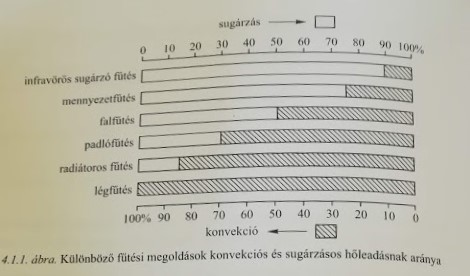
\includegraphics[width=8cm]{figures/konvrad}
	\caption{Alacsony hőmérsékletű fűtés és magas hőmérsékletű hűtés c. könyv ábrája}
		%\footnote{Jan Babiak, rehva Guidebook No.7}
\end{figure}


A levegő hőmérsékletére ezek a következőképp hatnak a leginkább:
\begin{itemize}[noitemsep,topsep=0pt,parsep=0pt,partopsep=0pt]
	\item a fűtőtestek konvektív és radiatív hőátadással is melegítik a környezetet
	\item a radiatív energiát a tárgyak, falak nyelik el, amik ezáltal felmelegszenek (mintegy kapacitásként lesz egy hőtároló tömeg, ami a fűtés kikapcsolásával fenntartja a hőmérsékletet / lassítja a hűlést)
	\item a fűtetlen falfelületek hűtik a szobát (külső hőmérséklet befolyása)
\end{itemize}

Így a kezdeti modellben azzal a feltételezéssel élek, hogy ezen kívül más hatás nem lép fel.

A modellben feltételezem, hogy a fűtőtest felületi hőmérsékletével tudunk beavatkozni. A modellben paraméter a fűtőtestek hőátadási tényezője és felülete. Zavarásként (?) hat a külső hőmérséklet értéke, amit mérni is tudunk. Kimenet a belső hőmérséklet (térben konstansnak véve azt / átlagolva a szoba levegőjére)

A modell felírásához a fűtőtest tulajdonságain kívül szükség van a szobában található levegő mennyiségére is. A zavarás hatását is fel kell írni, azaz hogy egy külső hőmérsékletváltozás hogyan jelenik meg a kimeneten. (Célszerű itt egy átviteli függvényt felírni először, szuperpozíciószerűen. A zavarás viszont nem a modell bemenetén és nem is a kimenetén hat.)

A felírandó átviteli függvények:

\begin{itemize}[noitemsep,topsep=0pt,parsep=0pt,partopsep=0pt]
	\item levegő felmelegedése konstans külső hőmérsékletet feltételezve, fűtőtest egységugrással
	\item levegő felmelegedése fűtés kikapcsolt állapota mellett, környezeti hőmérséklet ugrásával
\end{itemize}

Ezeket ráadtam a rendszerre és két bemenetű, egy kimenetű rendszerként identifikáltam.

%\pagebreak


%\subsubsection{Modellparaméterek}

\subsection{-----}

Fűtési típusok szerint:

\begin{itemize}[noitemsep,topsep=0pt,parsep=0pt,partopsep=0pt]
	\item radiátoros fűtés hőátvitele
	\item padlófűtés hőátvitele
\end{itemize}

A fentiekre különböző értékű lesz a 

\begin{itemize}[noitemsep,topsep=0pt,parsep=0pt,partopsep=0pt]
	\item hőátadási tényező
	\item hőtároló tömeg
	\item költségfüggvény?
	\item előremenő vízhőmérséklet és ezzel a leadott teljesítmény maximumértéke
\end{itemize}

ami így eltérő ház-modelleket fog eredményezni.










\pagebreak